\documentclass{article}   

\usepackage{geometry}
\usepackage{qtree}
\usepackage[square,numbers]{natbib}
% \usepackage{cite}  
\geometry{a4paper}

\usepackage[]{algorithm2e}
\usepackage{amsthm}
\newtheorem{theorem}{Theorem}[section]
\newtheorem{corollary}{Corollary}[theorem]
\newtheorem{example}{Example}
\newtheorem{lemma}[theorem]{Lemma}
\usepackage{rotating}
\usepackage[utf8]{inputenc}
\usepackage[T1]{fontenc}    % use 8-bit T1 fonts
\usepackage{lmodern}
\usepackage{hyperref}       % hyperlinks
\usepackage{lipsum}

%\usepackage[dvipsnames]{xcolor}
\usepackage{color, colortbl}

\definecolor{Gray}{gray}{0.9}
\definecolor{goldenpoppy}{rgb}{0.99, 0.76, 0.0}
\definecolor{goldenrod}{rgb}{0.85, 0.65, 0.13}

\usepackage[protrusion=true,expansion=true]{microtype}

\usepackage{amssymb}
\usepackage{amsfonts}
\usepackage{booktabs}
\usepackage{eqnarray,amsmath}
\usepackage[table]{xcolor}

\usepackage{listings}
\usepackage{dirtytalk}

\usepackage{rotating}
\usepackage{caption}

%% if you use PostScript figures in your article
%% use the graphics package for simple commands
\usepackage{graphics}


%% or use the graphicx package for more complicated commands
\usepackage{graphicx}


\usepackage{indentfirst}
\usepackage[utf8]{inputenc}
 \usepackage{subcaption}

 
\usepackage{xspace,color}
\usepackage{url}

\usepackage[export]{adjustbox}

\usepackage{listings}
\usepackage{xcolor}

\definecolor{codegreen}{rgb}{0,0.6,0}
\definecolor{codegray}{rgb}{0.5,0.5,0.5}
\definecolor{codepurple}{rgb}{0.58,0,0.82}
\definecolor{backcolour}{rgb}{0.95,0.95,0.92}

\lstdefinestyle{mystyle}{
    backgroundcolor=\color{backcolour},   
    commentstyle=\color{codegreen},
    keywordstyle=\color{magenta},
    numberstyle=\tiny\color{codegray},
    stringstyle=\color{codepurple},
    basicstyle=\ttfamily\footnotesize,
    breakatwhitespace=false,         
    breaklines=true,                 
    captionpos=b,                    
    keepspaces=true,                 
    numbers=left,                    
    numbersep=5pt,                  
    showspaces=false,                
    showstringspaces=false,
    showtabs=false,                  
    tabsize=2
}

\lstset{style=mystyle}

\newcommand{\ri}[1]{\lstinline{#1}}  %% Short for 'R inline'

\lstset{language=R}             % Set R to default language


%https://tex.stackexchange.com/questions/96825/nicely-formatted-where-statement-for-maths
 \newenvironment{where}{\noindent{}where\begin{itemize}}{\end{itemize}}
 \renewcommand*\descriptionlabel[1]{\hspace\leftmargin$#1$}
 
 %\newtheorem{theorem}{Theorem}[section]
%\newtheorem{corollary}{Corollary}[theorem]
%\newtheorem{lemma}[theorem]{Lemma}


\lstset{escapeinside={<@}{@>}}
% please place your own definitions here and don't use \def but
% \newcommand{}{}
%
% Insert the name of "your journal" with
% \journalname{myjournal}
%
\begin{document}

\title{%
  Practice 14: Central Limit Theorem. } %\\~\\
  %\Large }
\author{Mayra Cristina Berrones Reyes 6291}

\maketitle

\section{Introduction}

The Central Limit Theorem (CLT) tells us that in many situations, when independent random variables are added with unknown distribution (it could be uniform, binomial or completely random), the sample means will approximate the normal distribution, such as a bell curve. \\

Often, the CLT is confused with \say{the law of large numbers}. This law states that as the size of a sample increases, the sample mean will become a more accurate estimate of the population mean. The main difference between the two theorems is that the law of large numbers pertains to a single sample, meanwhile, the CLT pertains to the distribution of sample means \cite{twds}. \\

As statistical significance goes, the CLT \cite{bot}:

\begin{itemize}
\item Helps us analyze data like hypothesis testing and constructing confidence intervals, because these methods assume the population is normally distributed, so we can treat the sampling distribution as normal according to the CLT.
\item When we increase the samples form the population, the standard deviation of sample means will decrease. This helps us estimate the population mean much more accurately.
\end{itemize}

The mean of the sample means is denoted as Equation \ref{eq1} and the standard deviation of the sample mean is denoted as Equation \ref{eq2}\\

\begin{eqnarray}
\label{eq1}
\mu_{\overline{x}} = \mu,
\end{eqnarray}

where,
\begin{itemize}
\item $\mu_{\overline{x}}$ is the mean of the sample means.
\item $\mu$ is the population mean.
\end{itemize}

\begin{eqnarray}
\label{eq2}
\sigma_{\overline{x}} = \frac{\sigma}{\sqrt{n}},
\end{eqnarray}

where,
\begin{itemize}
\item $\sigma_{\overline{x}}$ is the standard deviation of the sample mean.
\item $\sigma$ is the population standard deviation.
\item $n$ is the sample size.
\end{itemize}

\subsection{Example: Die roll}
 Following similar steps as the practice of Law of Large Numbers (LLN), to further analyze and understand the CLT, we use the example of the dice and with code in R \ref{lol}. \\
 
  A fair die can be modeled with a discrete random variable with outcome 1 through 6, each with the equal probability of $\frac{1}{6}$. The expected value is $\frac{1+2+3+4+5+6}{6} =3.5$. In this experiment we are going to simulate throwing a fair die 10,000 times where we first have as a result Figure \ref{fig1}. \\

\begin{figure}[]
\centering
  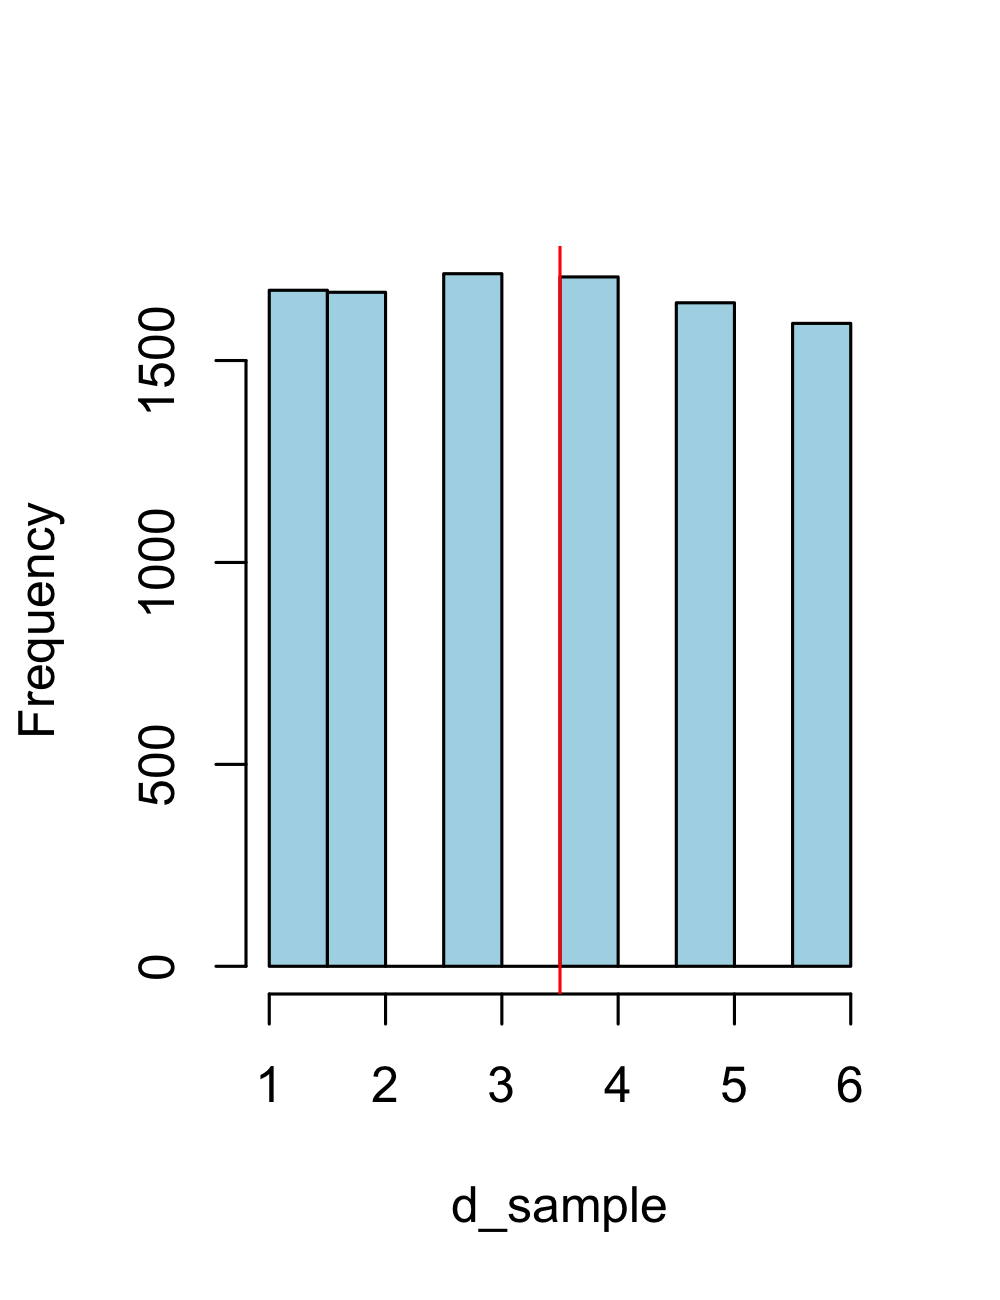
\includegraphics[width=.4\linewidth]{Ej14_dice.png} 
   \caption{Histogram of the frequency of each outcome.} 
\label{fig1}
\end{figure}


\begin{lstlisting}[language=R, caption=R extract of the code used to perform the dice experiment, label = lol ]
png("Ej14_dice.png", width = 1000, height = 1300, res = 300)
d_sample <- sample(1:6,10000, replace= TRUE)
hist(d_sample, col = "light blue",main="")
abline(v=3.5, col = "red",lty=1)
dev.off()

x30 <- c()
x100 <- c()
x1000 <- c()
k =10000
for ( i in 1:k){
  x30[i] = mean(sample(1:6,30, replace = TRUE))
  x100[i] = mean(sample(1:6,100, replace = TRUE))
  x1000[i] = mean(sample(1:6,1000, replace = TRUE))
}

png("Ej14_dice1.png", width = 1000, height = 1300, res = 300)
hist(x30, col ="light blue",main="",xlab ="die roll")
abline(v = mean(x30), col = "blue")
dev.off()

png("Ej14_dice2.png", width = 1000, height = 1300, res = 300)
hist(x100, col ="pink", main="",xlab ="die roll")
abline(v = mean(x100), col = "red")
dev.off()

png("Ej14_dice3.png", width = 1000, height = 1300, res = 300)
hist(x1000, col ="orange",main="",xlab ="die roll")
abline(v = mean(x1000), col = "red")
dev.off()

\end{lstlisting}

We will take samples of size 10, from the above 10,000 observations of the outcome of die roll. From this, we will take the arithmetic mean and try to plot the mean of sample. This procedure will be reproduced  k times (in this case k= 10,000). \\

By theory , we know as the sample increases, we get better bell shaped curve. As the n approaches infinity , we get a normal distribution. We will achieve this by increasing the sample size to 30, 100 and 1,000, and the results can be seen in Figure \ref{fig2}.\\

\begin{figure}[]
\begin{subfigure}{.5\textwidth}
  \centering
  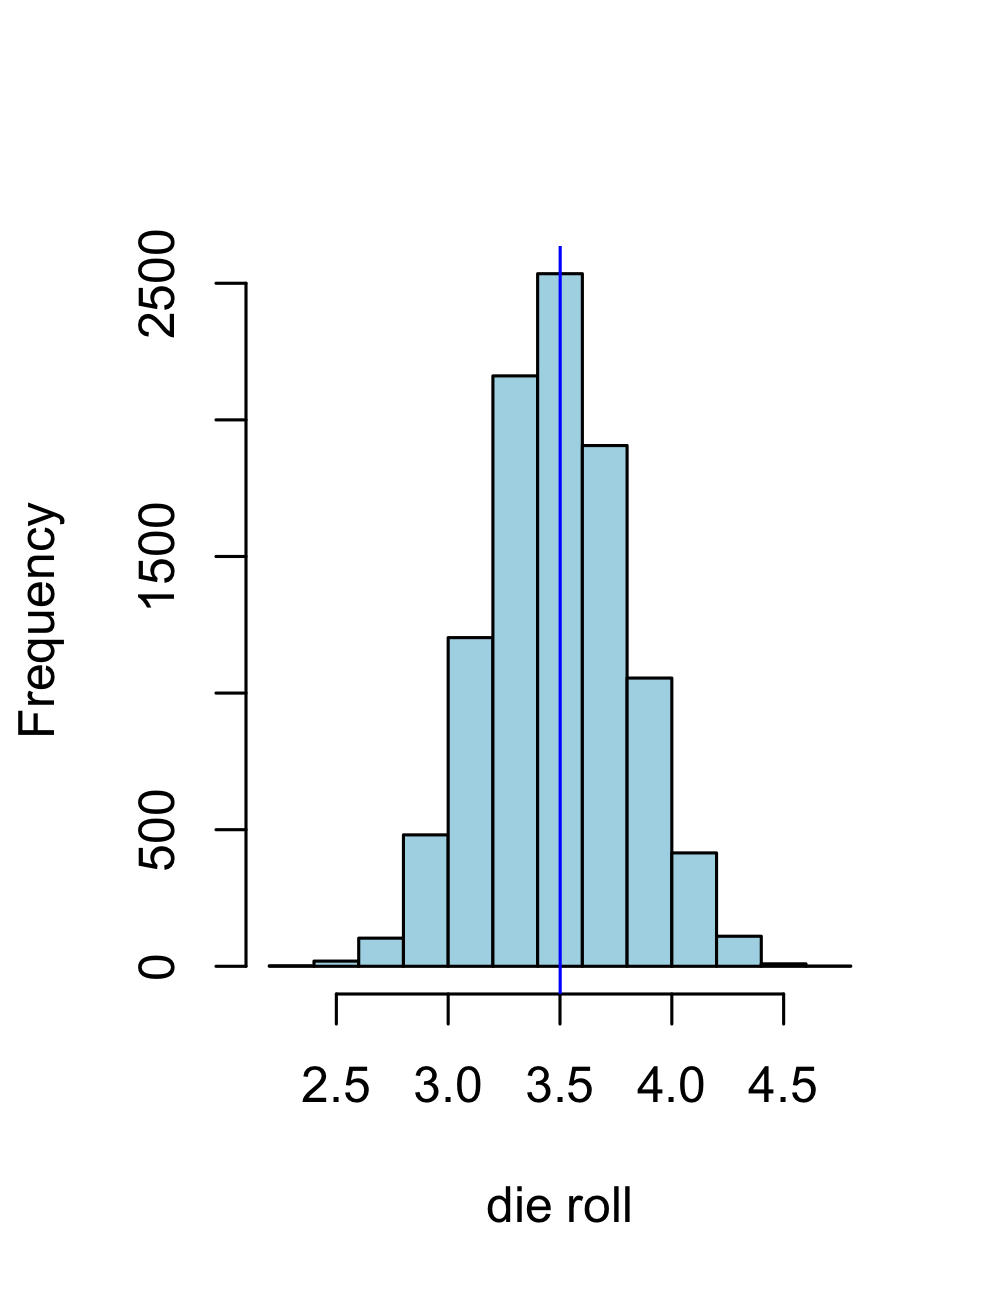
\includegraphics[width=.9\linewidth, left]{Ej14_dice1.png}  
  \caption{n = 30}
  \label{sb2-1}
\end{subfigure}\hspace{5mm}%
\begin{subfigure}{.5\textwidth}
  \centering
  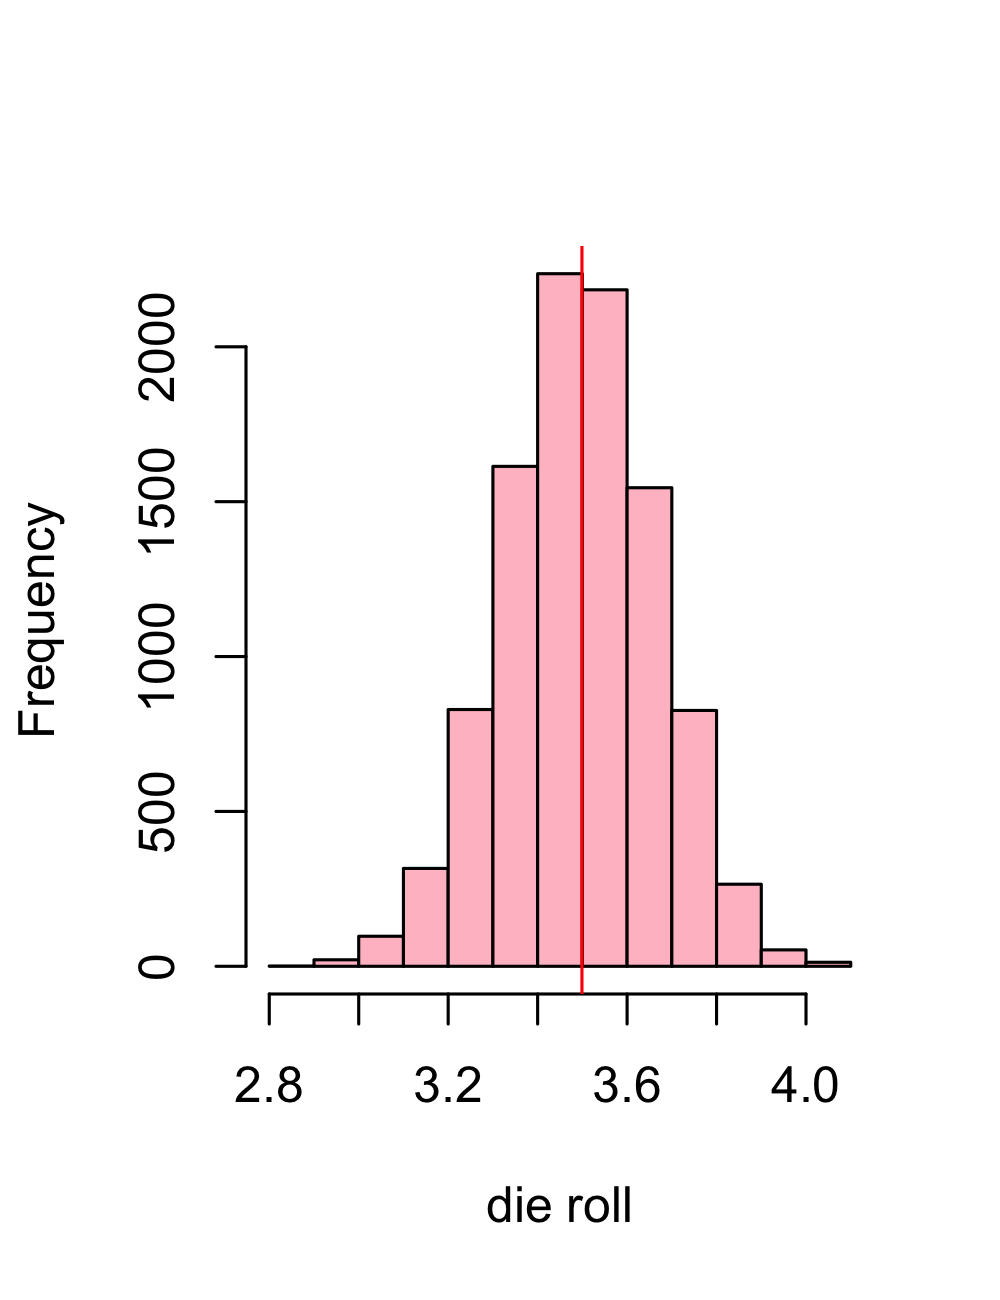
\includegraphics[width=.9\linewidth]{Ej14_dice2.png}  
  \caption{n = 100}
  \label{sb2-2}
\end{subfigure}\hspace{5mm}%
\newline
\begin{subfigure}{1\textwidth}
  \centering
  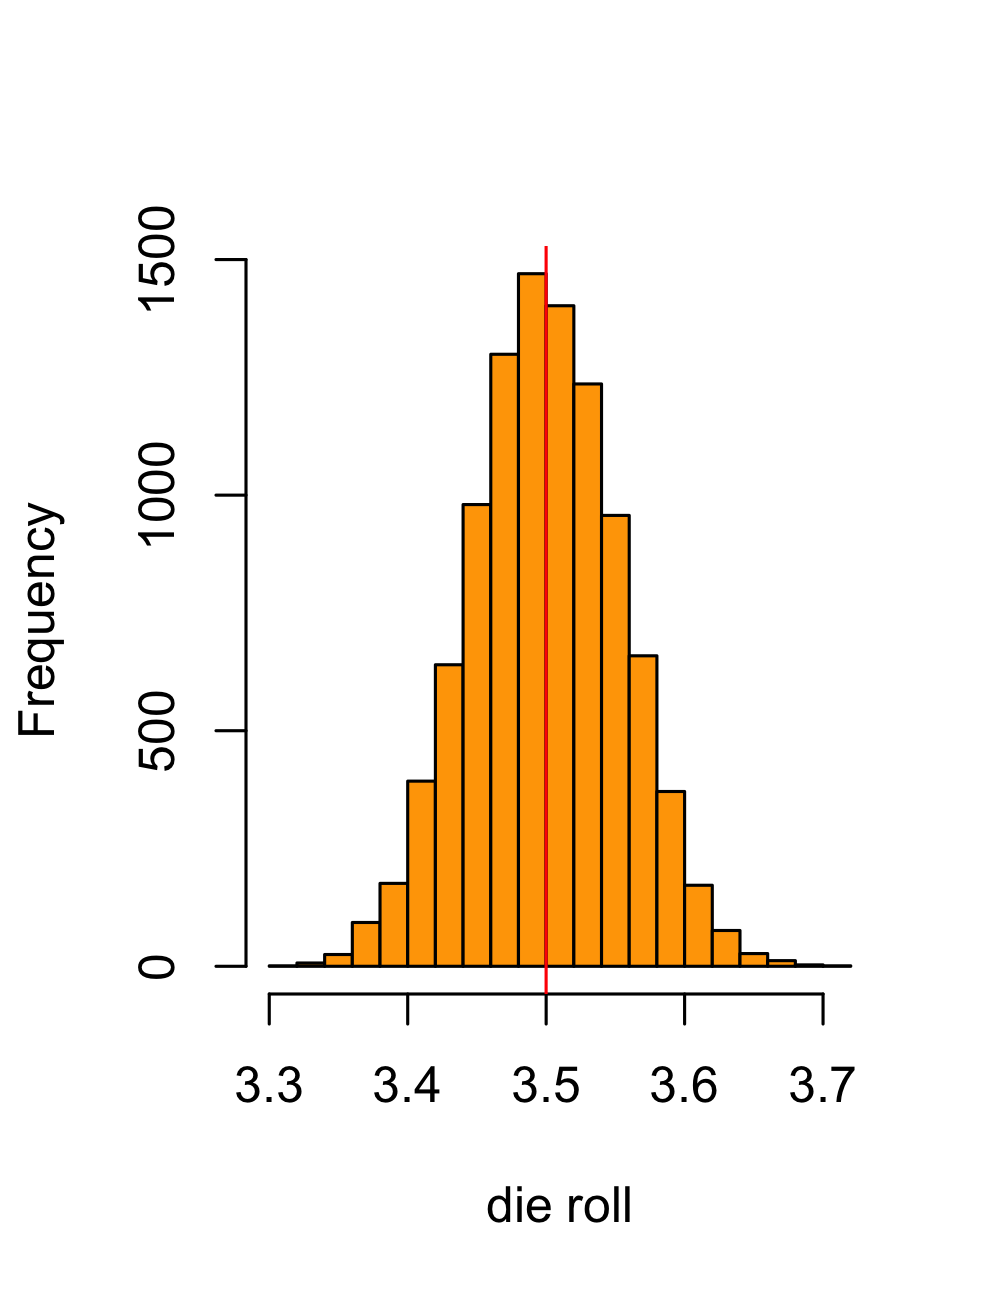
\includegraphics[width=.5\linewidth, center]{Ej14_dice3.png}  
  \caption{n = 1,000}
  \label{sb2-3}
\end{subfigure}
	\caption{Different parameters for the dice experiment performed in \texttt{R}.}
\label{fig2}
\end{figure}
\clearpage


\section{Applications of Central Limit Theorem in Machine Learning}

The CLT has important implications in applied machine learning. The theorem does inform the solution to linear algorithms such as linear regression, but not exotic methods like artificial neural networks that are solved using numerical optimization methods. Instead for these type of methods, we must use experiments to observe and record the behavior of the algorithms and use statistical methods to interpret their results. \\

For the significance test, we can make comparisons of the performance of one model against another model. In this case, we can use the tools of statistical significance to estimate the likelihood that the two samples of model skill scores were taken from the same or a different distribution of model scores. If it looks like the samples were drawn from the same population, then we assume there is no difference between the models, and any differences are due to statistical noise.\\

Another example is when we have trained a final model in machine learning, we want to make a guess about how good the model is expected to be in practice. This can be called a confidence interval. We can develop multiple independent evaluations of a model accuracy to result in a population of model accuracy estimates. The mean of these estimates will is regarded as the error of the true estimate of the model accuracy on the problem.\\

To illustrate this, we can actually take the example of the dice, and verify the standard error on each of the experiments seen on Figure \ref{fig2}.\\

For that example we have the variance of rolling a fair die equal to 2.92 and the standard deviation to 1.71, so we have the results in Table \ref{tab1}. In that table we can see, as the sample increases, the error gets smaller and smaller. \\


\begin{table}[]
\centering
\caption{Calculation of the standard error of the dice example.}\label{tab1}
\begin{tabular}{|c|c|c|}
\toprule
        \multicolumn{3}{|c|}{{{\bfseries Sample size}}} \\
\midrule  
    10      &  100 &    1,000   \\
    \midrule
$\sigma_{\overline{x}} = \frac{1.71}{\sqrt{10}} = 0.54$      &  $\sigma_{\overline{x}} = \frac{1.71}{\sqrt{100}} = 0.17$  &   $\sigma_{\overline{x}} = \frac{1.71}{\sqrt{1000}} = 0.05$    \\
\bottomrule
\end{tabular}
\end{table}

\section{Conclusion}

In this case with the CLT definition, a part of the process of training a Neural Network comes to mind. When training the models used for our investigation of the thesis, we focused on comparing the efficiency and accuracy of the models. In the training process, there is a sort of monitoring of the results and development of the model. Similar to what we did here, we chose a set number of iterations in which our models are to be trained. This iterations are also divided in epochs, that are a form of larger way to see the iterations and the slow process of improving the accuracy of your model.\\

The way it improves is dependent of the loss function you choose. In our case, we chose the binary cross-entropy (specifically for the type of data we had) and the main goal is to reduce the loss function a close to zero as we can, and have the accuracy as close to 1. This is the part of the process that most resonated while reading for examples, because of the way we look for one part of the process to be as close as zero and the other to converge to 1 (this part more so in the Law of Large Numbers).\\

In Figure \ref{final} we have a plot of the loss and accuracy pf the best models trained for the experimentation of our thesis. As we can see, in the best models, the accuracy is close to one in the last epoch, and the loss is closest to zero.\\

\begin{figure}[]
\centering
  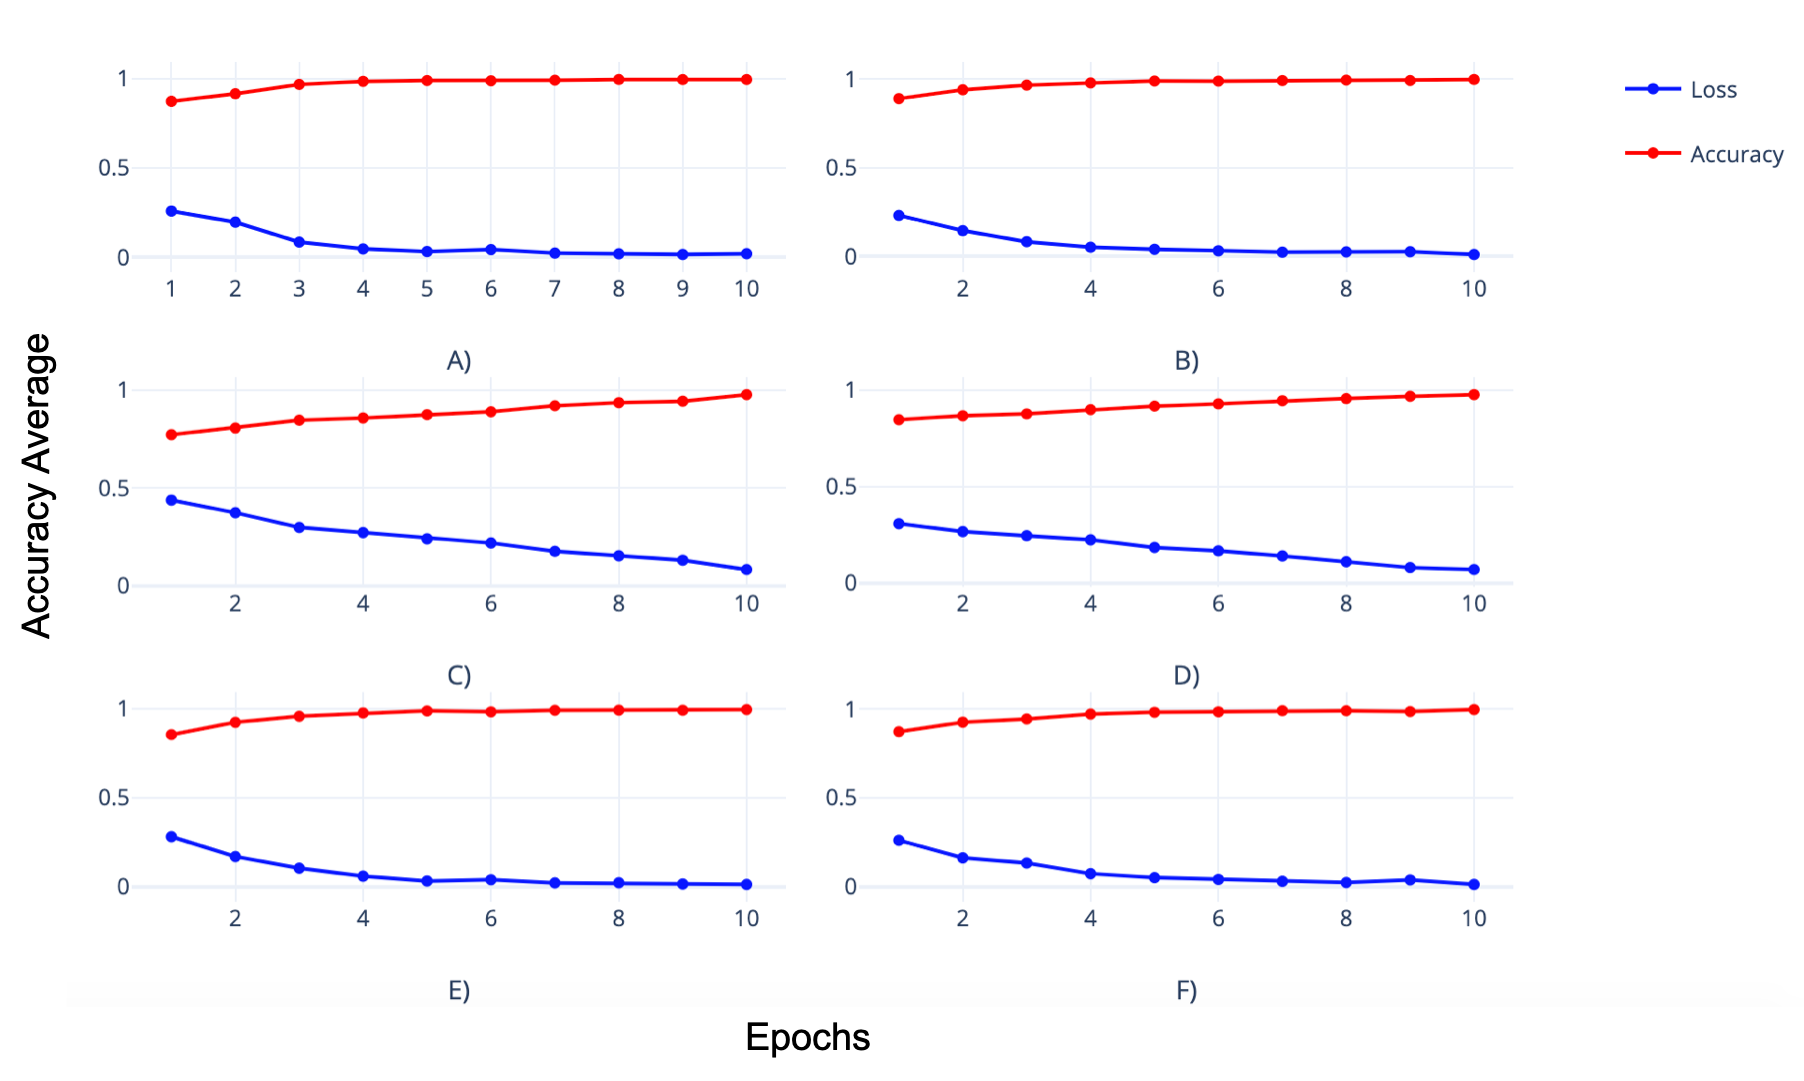
\includegraphics[width=1\linewidth]{lossfianl.png} 
   \caption{Loss and accuracy of the best models.} 
\label{final}
\end{figure}



In conclusion, understanding the central limit theorem is important when it comes to trusting the validity of the results of the models we train and assessing the precision of the estimated accuracy it gives. \\

\bibliographystyle{plainnat}
\bibliography{tarea14}


 
\end{document}